\documentclass{article}

\usepackage{multicol}


\usepackage{graphicx}% to include pdf image from matplotlib (vectorized)
\usepackage{subcaption}% to have plots with subimages
\usepackage{cite}
\usepackage{geometry}

\geometry{a4paper, left=0.5in,top=0.5in, right=0.5in, bottom = 0.8in}
\renewcommand{\familydefault}{\sfdefault}% make sans-serif font
%\setlength{\parindent}{0pt} % remove standard indentation

\usepackage{array}
\newcolumntype{P}[1]{>{\centering\arraybackslash}p{#1}}


\title{Project Rainy Day}
\date{2018}
\author{Alexander Hartenstein}

\begin{document}
	\maketitle


	\section{Requirements}
	We are working with an elementary school to develop and educational that allows students to interact with educational content projected by a projector onto the floor. Three dimensional sensors provided by a Kinect sensor allow movement to be translated into gameplay. The objective of this game is to facilitate learning through gameplay.
	\subsection{Functional Requirements}

\begin{enumerate}
	\item The system must allow the loading of educational content, in this case with the use of .csv files with key/value pairs.
	\item The system must include game play execution.
	\item The system must allow the setting of game parameters through a GUI.
	\item The system must connect with the Kinect hardware.
	\item The system must translate user movement into controls for game play.
	\item The system must update player scores as gameplay progresses.
	\item The system must update the graphical user interface to reflect game play.
	\item The system must save game state to allow for replaying and recovering from system failure.
\end{enumerate}
	\subsection{Non-Functional Requirements}

\begin{enumerate}
	\item System reaction time after player movement must be < 1s
	\item System should store up to 10,000 student ids but allow only maximally four players to play at one time.
	\item System should have be playable with one kinect and one projector.
	\item System should be playable with a minimum of 16 game cards (4x4 grid)
\end{enumerate}
	\subsection{Access Permission}

\begin{itemize}
\item Systemadmin: system maintenance has full access
\item Teacher: Gameadmin has access to GUI can Read/Write
\item Active player (Student): Can write
\item Passive player (Student): no access cant write/read
\end{itemize}
	\subsection{Glossary}

\begin{enumerate}
	\item Memory : a game in which a grid of blank boxes is displayed. Players select two cards in consecutive order a card, which 'flips' the card to reveal the 'content side'. If the two 'content sides' match, the player receives a point. The player with the most matches wins. If the two 'content sides' do not match, the two revealed cards flip back to the 'blank side', and the next players flip two cards.
	\item Content side : The side of a 'card' which contains information fed from teacher input data, which must be matched with another 'content side' during gameplay.
	\item Player : a student who is involved in active game play.
	\item Teams : two players that act as a single unit, collaborating on an x, y axis to select a single 'card' to be flipped.
	\item Game administrator : in this case, the teacher who is responsible for selecting game parameters such as time limits and number players/teams.
	\item Kinect : sensor from microsoft with depth sensors and rgb camera which is used as a game controller to register player movement/selections
	\item Depth sensors : allows to register three dimensional movement. Rather than rgb values at each pixel, a milimeter depth value is returned at each pixel value.
	\item Game content : a csv table allowing for input of education content by teachers at the school. Each row represents a pair of memory cards which must be matched during game play.
\end{enumerate}

	\begin{figure}[h!]
	  \centering
	    \includegraphics[width=\textwidth]{components/usecasediagram.png}
	    \caption{Use Case Diagram}
	    \label{fig:use_case_diagram}
	\end{figure}


	\begin{figure}[h!]
	  \centering
	    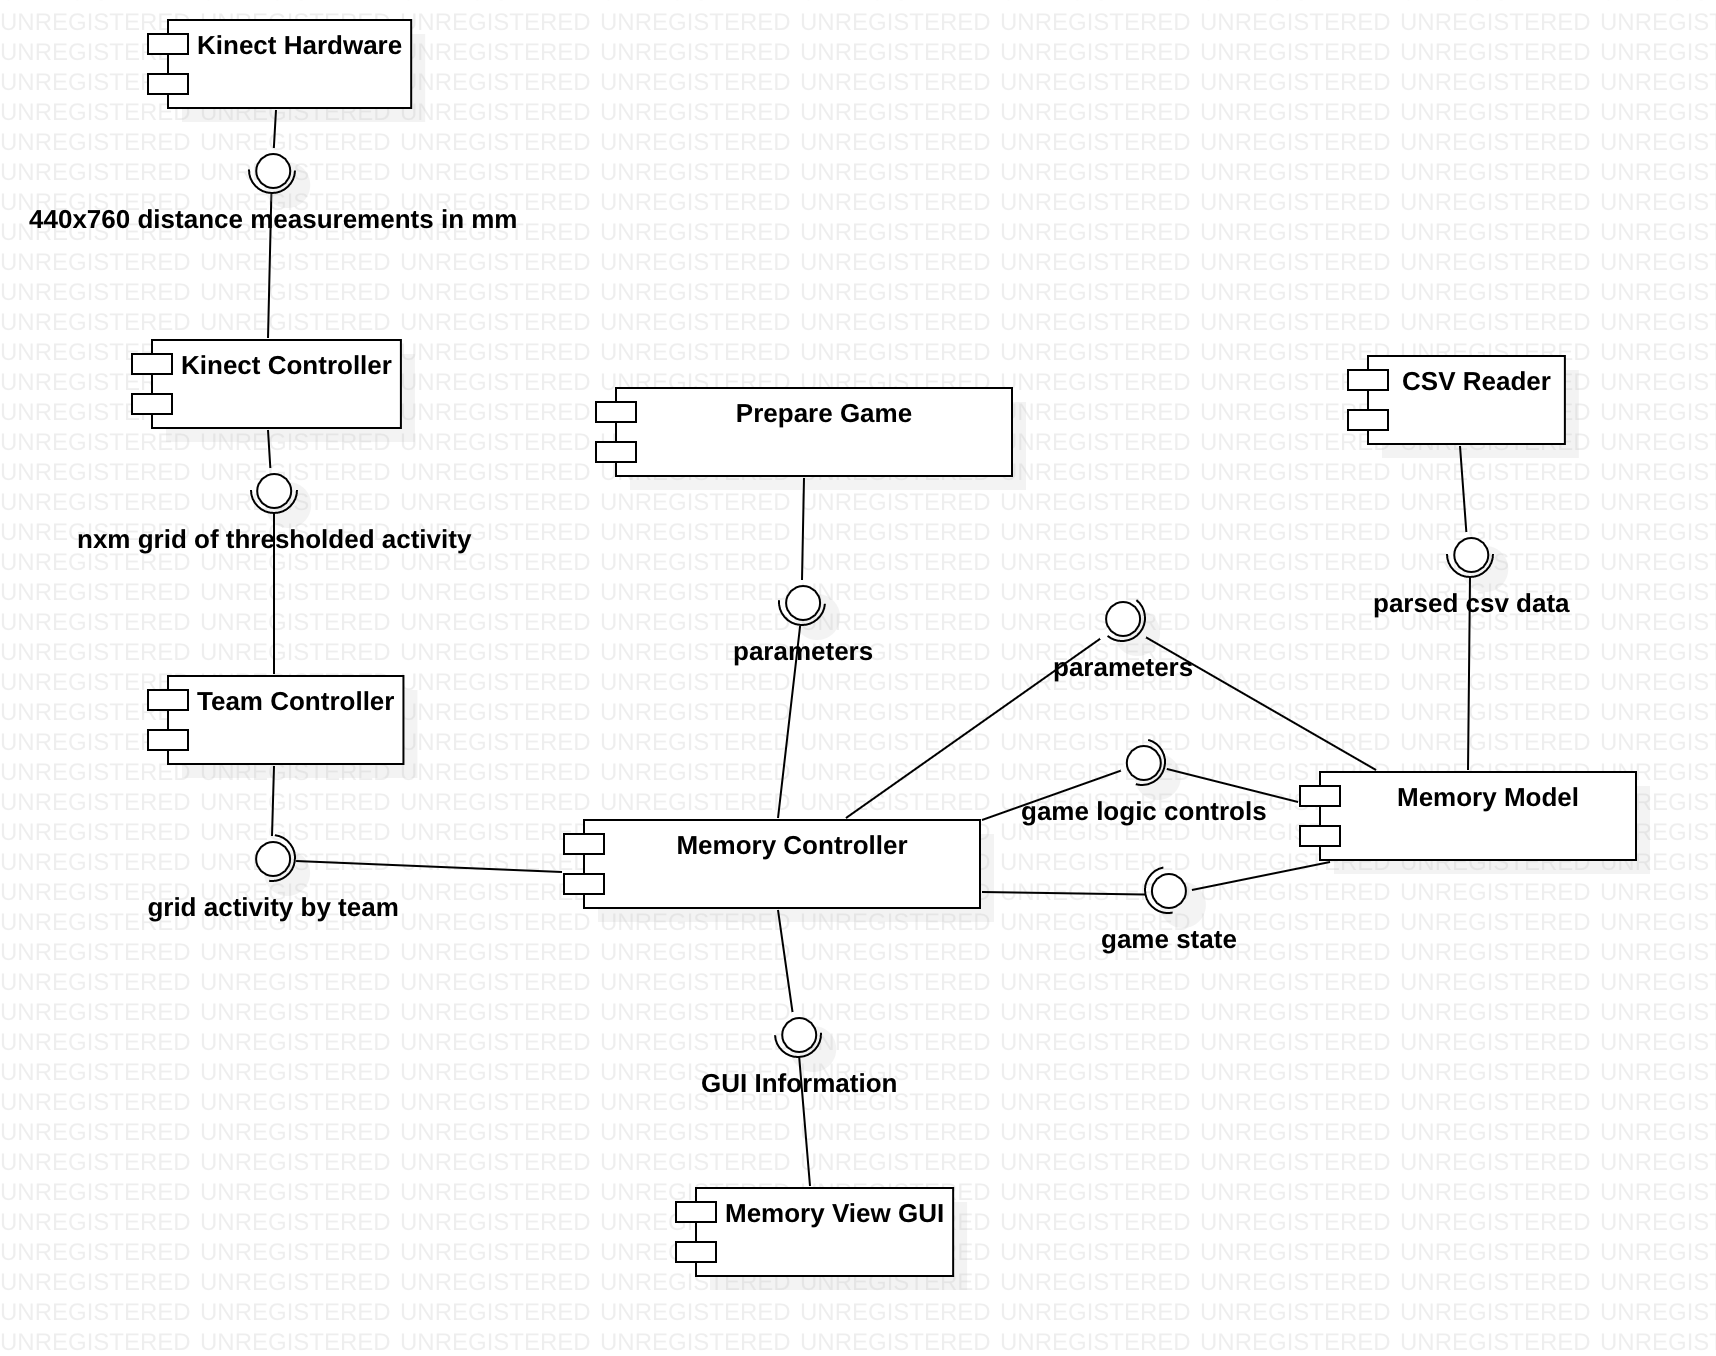
\includegraphics[width=\textwidth]{components/componentDiagram.png}
	    \caption{Component Diagram}
	    \label{fig:component_diagram}
	\end{figure}






\end{document}